% Machine-Verifiable Item Models for Geometry Diagram Generation
%
% NCME submission. NCME uses the ACL format, so we typeset with the official
% ACL style (acl.sty).
%   [final] => ACL two-column camera-ready layout: no line numbers, no page
%   numbers, real author names (AIME-Con proceedings require all three).
%   For a line-numbered anonymous review copy, switch [final] -> [review].
%
% Build with pdfLaTeX (make) or Overleaf.

\documentclass[11pt]{article}
\usepackage[final]{acl}

\usepackage{times}
\usepackage{latexsym}
\usepackage[T1]{fontenc}
\usepackage[utf8]{inputenc}
\usepackage{microtype}
% \usepackage{inconsolata}   % optional ACL typewriter font; omit if not installed
\usepackage{graphicx}

% Project macros + math/tikz/tables. acl.sty already provides xcolor, natbib,
% hyperref, geometry, caption, url, so those are not reloaded in preamble.tex.
% Preamble — NCME submission "Machine-Verifiable Item Models for Geometry Diagram Generation" (ACL format).
% Loaded AFTER \usepackage[preprint]{acl} in main.tex, so acl.sty has already
% provided xcolor, natbib (author-year), hyperref, geometry, caption, url.
% Add only what ACL does not provide, plus the project macros.

\usepackage{amsmath,amssymb}
\usepackage{booktabs}
\usepackage{array}

\usepackage{tikz}
\usetikzlibrary{positioning,arrows.meta,calc}

\usepackage{xspace}
\usepackage{enumitem}
\setlist[itemize]{itemsep=3pt, topsep=4pt}

% cleveref last (after hyperref, which acl.sty loads)
\usepackage[capitalize,noabbrev]{cleveref}

% --- macros ---
\newcommand{\GeoGen}{\textsc{GeoGen}\xspace}
\newcommand{\GeoGenBench}{\textsc{GeoGenBench}\xspace}
\newcommand{\propname}[1]{\texttt{#1}}


\title{Machine-Verifiable Item Models for Geometry Diagram Generation}
\author{Mei Chen \qquad Gordon Stein \\
  Renaissance Philanthropy}

\begin{document}
\maketitle

\begin{abstract}
Language models can draw geometry diagrams that look right but are actually
wrong. We found that a more reliable way to generate diagrams is to have the model
first describe the construction, then have a
geometry engine compute every point and check the result against the stated
geometric requirements, and only then render the diagram. Because the
checklist for each prompt is written once, when the prompt is, and applied by
the engine, no one grades a diagram by hand. We tested this on 600 benchmark prompts across six
models and found that structured generation raised pass rates for every model
that could run it. We also had two human graders check the grader. They showed
it is lenient in one direction: it passed 36 of 200 diagrams they failed and
failed none the human graders passed.
\end{abstract}


\section{Introduction}
\label{sec:motivation}

\emph{Automatic item generation} (AIG) can reduce the workload of producing new test items and their answer keys. In template-based AIG, an author writes a single template, or \emph{item model}, from which a computer generates many items, each carrying its own answer key \citep{bejar2002generative,gierl2013aig}. AIG has been applied mainly to items built from text. Items whose response is a \emph{picture} have been harder to reach. In K--12 mathematics, the picture that matters most is the geometry diagram.

Producing a correct diagram is harder than it appears. Consider a simple request:

\begin{quote}
\emph{``Draw an acute triangle $ABC$ with $\angle A = 60^\circ$ and $\angle B = 70^\circ$, then draw the altitude from $C$, meeting $AB$ at $H$.''}
\end{quote}

To be correct, the drawing must satisfy several requirements \emph{exactly}. Angle $A$ is $60^\circ$. The point $H$ lies on the segment $AB$, not past its end. The altitude meets $AB$ at a true right angle. A model that draws directly has no step at which the drawing is checked against these requirements. Whether they hold is a matter of chance. When they fail, they fail silently.

The same exactness makes such diagrams hard to score. Most geometry benchmarks pose the reverse task. They show the model a finished diagram and ask a question about it \citep{lu2021intergps,lu2024mathvista}. They do not ask whether a model can \emph{produce} a correct figure. The benchmarks that do score generated pictures were built for everyday images. They rely on a model-based judge that inspects the output \citep{huang2025t2icompbenchpp,wang2025genexam}. A judge can report that a shape \emph{resembles} a right triangle. It cannot certify that an angle is exactly $90^\circ$. For geometry diagrams, then, neither producing the item nor scoring it is straightforward.

Our approach removes both the guessing and the inspection. The model describes the construction in words: ``$H$ is the foot of the perpendicular from $C$ to $AB$.'' A geometry engine then computes the exact coordinates. The model decides \emph{what} to build. The engine determines \emph{where} every point lies. This single change addresses both problems.

\begin{itemize}
\item \textbf{Better drawings.} A solver performs the computation, so a right angle is exactly right rather than approximately so.
\item \textbf{Automatic scoring.} The finished figure is a set of exact coordinates, so each requirement can be checked directly. The question ``is this angle $90^\circ$?'' replaces a judge's impression of the picture.
\end{itemize}

That is this paper's contribution: a \emph{machine-verifiable item-model framework} for geometry diagrams. One item model emits both the prompt and a \emph{computed} answer key. The key is a machine-checkable list of geometric requirements. The figure produced in response is verified against that key. We make two empirical claims and are deliberate about their strength. Structured construction improves how often models get the geometry right (\cref{sec:benchmark}). Human validation shows the automatic score runs optimistic, so it is not yet a validated high-stakes score (\cref{sec:scoring}). A fuller leaderboard and cost analysis appear in a companion paper. Here the benchmark is evidence for these two claims, not the contribution itself.

The rest of the paper describes how the model describes a diagram (\cref{sec:pipeline}), how scoring follows from that same description (\cref{sec:scoring}), what we found on six large models (\cref{sec:benchmark}), and why this matters for educational measurement (\cref{sec:measurement}).

\section{How the model draws a diagram}
\label{sec:pipeline}

A request becomes a picture in four steps, shown in \cref{fig:trace}. The model writes a short, structured \emph{description} of the construction; a geometry engine turns that description into exact coordinates; and a renderer turns the coordinates into a drawing. The important idea is the division of labour: \textbf{the model decides what to build, and the engine decides where the points go.} The model never writes a number.

\begin{figure*}[t]
\centering
\resizebox{\textwidth}{!}{%
\begin{tikzpicture}[
  font=\scriptsize,
  box/.style={draw, rounded corners, align=left, inner sep=3pt, text width=24mm, minimum height=23mm, anchor=center},
  code/.style={box, fill=blue!4, font=\ttfamily\tiny},
  hd/.style={font=\scriptsize\bfseries},
  ar/.style={-{Stealth[length=2mm]}, thick, gray!55!black},
  arl/.style={font=\tiny\itshape, color=gray!45!black, align=center}
]
\def\dx{3.5}
\node[box, fill=yellow!10] (p) at (0,0) {\scriptsize ``Draw an acute triangle $ABC$ with $\angle A{=}60^\circ$, $\angle B{=}70^\circ$; construct the altitude from $C$ meeting $AB$ at $H$.''};
\node[code] (ir) at (\dx,0) {A, B: free\\C: by\_angles(\\\ \ A, B, 60, 70)\\H: inter(\\\ \ line A--B,\\\ \ perp thru C)\\seg C--H\\\textbf{check}\\\ \ right\_angle(C,H,A)};
\node[code] (sp) at (2*\dx,0) {A = (0, 0)\\B = (5, 0)\\C = (3.07, 5.31)\\H = (3.07, 0)};
\node[code] (tk) at (3*\dx,0) {\textbackslash tkzDefPoint\\\ \ (0,0)\{A\}\ \dots\\\textbackslash tkzDrawPolygon\\\ \ (A,B,C)\\\textbackslash tkzDrawSegment\\\ \ (C,H)};
\node[box, fill=green!6] (svg) at (4*\dx,0) {\centering
  \begin{tikzpicture}[scale=0.30]
    \coordinate (A) at (0,0);\coordinate (B) at (5,0);
    \coordinate (C) at (3.07,5.31);\coordinate (H) at (3.07,0);
    \draw[thick] (A)--(B)--(C)--cycle;
    \draw[densely dashed] (C)--(H);
    \draw (H)++(-0.55,0)--++(0,0.55)--++(0.55,0);
    \foreach \q in {A,B,C,H}{\fill (\q) circle (5pt);}
    \node[below left=-2pt,font=\tiny]  at (A) {$A$};
    \node[below right=-2pt,font=\tiny] at (B) {$B$};
    \node[above=-2pt,font=\tiny]       at (C) {$C$};
    \node[below right=-2pt,font=\tiny] at (H) {$H$};
  \end{tikzpicture}};
\foreach \n/\t in {p/{Prompt}, ir/{Description (IR)}, sp/{Coordinates}, tk/{Drawing code}, svg/{Figure}}{
  \node[hd, above=1.5mm of \n] {\t};}
\draw[ar] (p)  -- (ir) node[arl, midway, above] {model\\describes};
\draw[ar] (ir) -- (sp) node[arl, midway, above] {engine\\solves};
\draw[ar] (sp) -- (tk) node[arl, midway, above] {emit};
\draw[ar] (tk) -- (svg) node[arl, midway, above] {render};
\end{tikzpicture}}
\caption{One request, start to finish. The model writes a description of the construction; the geometry engine solves it for exact coordinates; the system emits drawing code and renders it. Because the model writes relationships (``$H$ is the foot of the perpendicular from $C$'') rather than numbers, the geometry is computed rather than guessed---and those same coordinates are what we grade against in \cref{sec:scoring}.}
\label{fig:trace}
\end{figure*}

\paragraph{Step 1: a description, not coordinates.}
The model fills in a simple, typed form---we call it the intermediate representation, or IR. The form offers about twenty kinds of building block: points, segments, lines, circles, polygons, and intersections. Each block names a \emph{relationship} rather than a position. A point can be ``the midpoint of $A$ and $B$,'' ``where these two lines cross,'' or ``the foot of the perpendicular from $C$.'' In our example the model writes ``$H$ is where line $AB$ meets the perpendicular to $AB$ through $C$''---never ``$H = (3.07, 0)$.'' Because the form is typed, obvious mistakes (a missing point, the wrong number of arguments) are caught right away, before any geometry is computed.

\paragraph{Step 2: the engine solves for the points.}
A geometry engine---we use SymPy, a symbolic-mathematics library---reads the description and works out the coordinates, handling the building blocks in dependency order. When a step is ambiguous (two circles cross at two points), the description simply says which one to keep (``the higher one''). The engine, not the model, produces every coordinate. This is what makes the right angle in our example \emph{exactly} $90^\circ$ rather than approximately so.

\paragraph{Step 3: render.}
From the exact coordinates the system writes standard drawing code and compiles it to an image. Fiddly details an author should not have to manage---such as clipping a line at the edge of the canvas---are handled automatically.

\paragraph{Two ways to drive it.}
The model can fill in the form directly, or it can use a short ``recipe'' language that names a construction---\texttt{perp\_bisector(A,B)}---which then expands into the same form. Either way, the description can carry its own requirements, tested \emph{before} the figure is drawn, so the model can catch a mistake and retry. We compare both against a plain baseline in which the model just writes drawing code by hand, with no engine and no checks; that baseline is how we measure what the structured approach is worth (\cref{sec:benchmark}).

\section{Automatic scoring from shared construction logic}
\label{sec:scoring}

Each item model writes two things at once: the prompt shown to the language model and the checklist used to score the diagram (\cref{fig:cogen}). Because the finished diagram is a set of coordinates, the engine can decide each check directly. ``Is the angle at $H$ a right angle?'' is settled by a single calculation on the coordinates. No judge is asked whether the picture appears square. This makes scoring inspectable and inexpensive. It does not make scoring complete. The checklist's validity still depends on whether it captures everything the prompt asks for and the visual conventions a reader expects. We examine both limits below.

\paragraph{The question and its answer key are written together.}
Each item and its answer key come from the \emph{same} short program. Because the two are emitted together, they are far less likely to drift apart through manual editing. Errors in the item model itself remain possible. An author can still omit a predicate, encode the wrong one, or write wording whose intended constraint the checklist does not fully capture. Re-running the item model with a new random seed produces a fresh, parallel item. The checklist is never shown to the language model while it works.

\begin{figure*}[t]
\centering
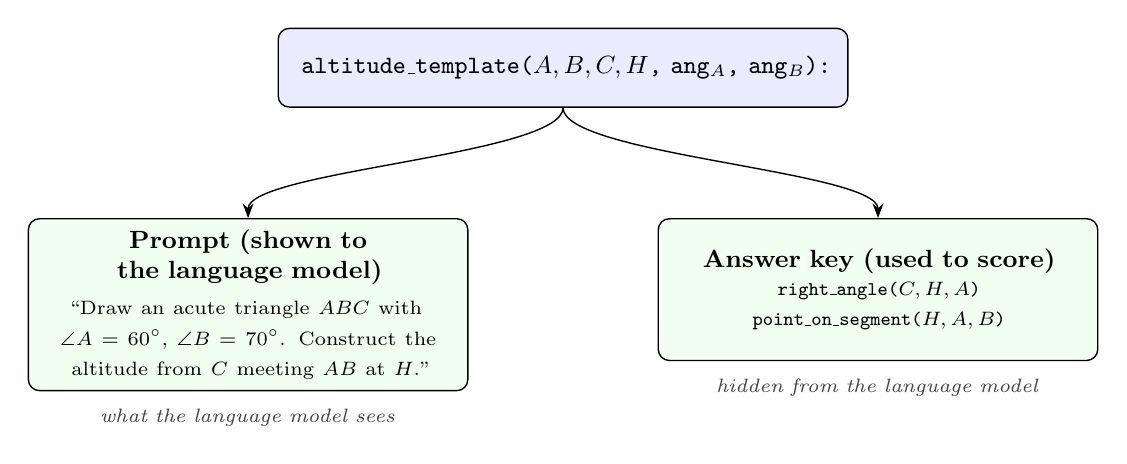
\begin{tikzpicture}[
    every node/.style={font=\small},
    func/.style={draw, rounded corners, fill=blue!8, align=center,
                 text width=70mm, minimum height=10mm, font=\ttfamily\small},
    outbox/.style={draw, rounded corners, fill=green!6, align=center,
                text width=53mm, minimum height=18mm, inner sep=4pt},
    role/.style={font=\scriptsize\itshape, color=gray!50!black, align=center},
    >=Stealth, line width=0.5pt
]
  \node[func] (fn) {altitude\_template($A,B,C,H$,\ ang$_A$,\ ang$_B$):};
  \node[outbox, anchor=north] (prompt) at ($(fn.south)+(-4.0,-1.4)$) {%
    \textbf{Prompt (shown to the language model)}\\[2pt]
    \scriptsize ``Draw an acute triangle $ABC$ with $\angle A = 60^{\circ}$, $\angle B = 70^{\circ}$.
    Construct the altitude from $C$ meeting $AB$ at $H$.''};
  \node[outbox, anchor=north] (rubric) at ($(fn.south)+(4.0,-1.4)$) {%
    \textbf{Answer key (used to score)}\\[2pt]
    \scriptsize\ttfamily right\_angle($C, H, A$)\\
    point\_on\_segment($H, A, B$)};
  \draw[->] (fn.south) .. controls +(0,-0.6) and +(0,0.6) .. (prompt.north);
  \draw[->] (fn.south) .. controls +(0,-0.6) and +(0,0.6) .. (rubric.north);
  \node[role, below=1mm of prompt, text width=53mm] {what the language model sees};
  \node[role, below=1mm of rubric, text width=53mm] {hidden from the language model};
\end{tikzpicture}
\caption{One item model writes both the question and its answer key. The two cannot drift apart through separate editing. An item model can still leave a check out. This key confirms the altitude but not the two stated angles. That gap is the main finding of the human study reported in this section.}
\label{fig:cogen}
\end{figure*}

\paragraph{A small, readable checklist.}
Each encoded requirement uses a small, fixed vocabulary of checks (\cref{tab:predicates}): right angle, midpoint, parallel lines, point on segment, and so on. There are 15 such checks in the current version. The construction is computed symbolically; each check is then decided numerically on the coordinates, within a small tolerance (\cref{sec:benchmark}). A diagram passes only if every check on its list passes. The list defines what the automatic scorer evaluates. It plays the role a specification plays in formal methods: a statement of what must hold, written so that a machine can check it. The check here is numeric and applied to one figure at a time, not a proof over all figures. For that reason we say \emph{verifiable} rather than \emph{verified}.

\begin{table}[t]
\centering
\footnotesize
\setlength{\tabcolsep}{4pt}
\begin{tabular}{@{}l p{0.5\columnwidth}@{}}
\toprule
\textbf{Check} & \textbf{What it confirms}\\
\midrule
\propname{right\_angle}                     & an angle is a right angle\\
\propname{midpoint}                         & a point is halfway along a segment\\
\propname{collinear} / \propname{parallel}  & points lie on a line / lines never meet\\
\propname{point\_on\_segment}               & a point lies between two endpoints\\
\propname{equal\_lengths}                   & two segments have equal length\\
\propname{angle\_equal}                     & an angle equals a stated value\\
\bottomrule
\end{tabular}
\caption{A sample of the 15 checks in the scoring vocabulary. Each is decided on the computed coordinates. An item's list of checks is what a passing answer must satisfy.}
\label{tab:predicates}
\end{table}

\paragraph{Does the automatic score match a human's?}
An automatic score is useful only if it agrees with a careful human grader, so we tested that agreement. We fixed a few blind spots found on an early pilot. We then ran a pre-registered study on a later run of the benchmark.\footnote{Protocol: \texttt{docs/human\_study\_protocol.md} in the code repository, \url{https://github.com/RenaissancePhilanthropy/geometry-diagram-generator}.} We set the bar in advance: the automatic score had to match the human verdict at Cohen's $\kappa \ge 0.70$, on a scale where $1.0$ is perfect agreement and $0$ is chance. Two graduate-level graders then scored 200 diagrams by hand, without seeing the automatic verdict. The 200 were drawn from that run stratified by automatic verdict: every uncertain and every rendered failing diagram, plus passes balanced across models, modes, and difficulty tiers. Each grader rated independently, and disagreements were then discussed to a single consensus verdict per diagram. We compare the automatic verdict with that consensus, both collapsed to pass or fail, with a partial human verdict counted as a fail.

We did not clear that bar. Agreement was moderate, Cohen's $\kappa = 0.46$, well short of the pre-registered $0.70$. We treat this as a central limitation. The disagreements run \emph{one way}. In 36 of the 200 cases the automatic scorer passed a diagram the graders failed. No automatic failure received a passing human verdict. That is the more serious direction once a score is read as a certificate of correctness, because every disagreement is a false positive. We therefore state it plainly: \textbf{the pass rates in \cref{sec:benchmark} may overestimate correctness}. Inspecting the 36 disagreements traced them to the checklist rather than to the ratings. They concentrate in items with an added construction, like our altitude, whose checklist confirms the construction but does not re-check the prompt's stated angles. The two graders agreed with \emph{each other} at the $0.70$ we had asked the scorer to reach. The fix is to add the missing numeric checks to those item models. That revision was not applied to the results reported here. Instead, \cref{sec:benchmark} reports, alongside each automatic pass rate, the share of automatic passes the graders confirmed, as a sensitivity calculation.

\paragraph{What the checks cannot see.}
That particular gap closes with more checks. A deeper one does not. The checks read the geometry, the coordinates, and nothing else. They never look at how the figure is drawn. A diagram can satisfy every requirement and still mislead a reader. A right-angle mark can be placed outside the corner. An angle can be labelled on the wrong side. A figure can pass every check and still be laid out so poorly that a reader cannot follow it. This is the converse of the language model-based judge in \cref{sec:motivation}. A judge sees how a picture looks but cannot check its geometry. Our checks test the geometry but cannot see how it looks. The two are complementary. The checks say whether the computed geometry is correct. Whether the drawing presents that geometry faithfully and clearly still requires visual review.

\section{Benchmark results}
\label{sec:benchmark}

Across the 600 item-model prompts of \GeoGenBench, the structured mode raised automatic pass rates for every model that could run both modes (\cref{tab:results}). \GeoGenBench holds 801 prompts, all scored by the checker of \cref{sec:scoring}: 600 generated from the item models described above, and 201 written from the topic scaffold of a K--12 mathematics curriculum~\citep{bluebonnet2024}. The results below cover the 600. The prompt set, item models, checker vocabulary, and rendered outputs are public, and so is the code.\footnote{Data: \url{https://huggingface.co/datasets/meix/geogenbench}. Code: the repository in footnote 1.} We ran six large models from three companies, each in two modes. The \emph{by-hand} mode has the language model write drawing code directly. The \emph{structured} mode has it fill in the description of \cref{sec:pipeline}. Each prompt was run three or more times, so a cell in \cref{tab:results} holds 1,800 to 2,861 generations, and a rate is the share of those generations that passed the automatic checker. The checker overestimated human acceptance in the validation sample (\cref{sec:scoring}), so these rates may overestimate correctness.

\paragraph{How we ran it.}
The by-hand mode asks the language model for TikZ drawing code. The structured mode asks for the typed form of \cref{sec:pipeline}. For the by-hand mode, an extractor recovers the coordinates from the TikZ source; output the extractor cannot parse counts as a failure. Both run at temperature $1.0$, the sampling setting that controls randomness, with no explicit limit on output length. Both have the same budget of up to three attempts. What differs is the retry trigger. The by-hand mode retries only when its code fails to render. The structured mode also retries when its description fails to compile or the figure breaks a check it declared. Those declared checks are the language model's own. The held-out scoring predicates generated by the item model, the ones we grade against, are never shown to the language model. The comparison is therefore between two complete workflows. The structured mode's feedback lets a model catch its own geometric mistakes, which the by-hand mode cannot, and its extra retries appear in its per-item cost. Each requirement is decided on the computed coordinates within an absolute tolerance of $\tau = 5\times10^{-3}$, applied to angles in radians and to lengths in coordinates normalised to $[-10, 10]$. The $600$ item-model prompts divide evenly across three difficulty tiers of $200$ each. They come from $30$ item models covering triangles, quadrilaterals, circles, segments, and lines, with $3.2$ requirements apiece on average. The $201$ curriculum prompts were drafted with a language model, with answer keys written by hand. They carry more requirements, $6.0$ on average. Cost per item is the input and output tokens of the prompt and its response, summed across any retries and priced at each vendor's published rates, then averaged over every prompt, failures included. Failures are dominated by wrong geometry, a requirement that does not hold, rather than by broken drawing code. The structured mode's remaining failures are mostly timeouts.

\begin{table}[t]
\centering
\footnotesize
\setlength{\tabcolsep}{5pt}
\begin{tabular}{@{}lrrr@{}}
\toprule
\textbf{Model} & \textbf{By hand} & \textbf{Structured} & \textbf{\$/item}\\
\midrule
GPT-5.5            & 91.9\% & \textbf{94.1\%} & 0.075\\
Claude Sonnet 4.6  & 81.2\% & 93.4\% & 0.088\\
Claude Opus 4.7    & 71.6\% & 93.3\% & 0.53\\
Claude Haiku 4.5   & 70.5\% & 75.3\% & 0.032\\
Gemini 2.5 Pro     & 58.4\% & 83.1\% & 0.050\\
Gemini 2.5 Flash   & 35.9\% & blocked & ---\\
\midrule
\emph{Confirmed by graders} & 75\% & 87\% & ---\\
\bottomrule
\end{tabular}
\caption{Share of generations \emph{passing the current automatic checker} over the $600$ item-model prompts, each run three or more times, in the by-hand mode and the structured mode, with the average cost of one structured generation in US dollars. The checker overestimated human acceptance in the validation sample (\cref{sec:scoring}), so these rates may overestimate correctness. The last row gives the share of automatic passes that human graders confirmed, pooled over models. Every model that could run the structured mode improves. The three strongest converge near $93$--$94\%$ despite a sevenfold difference in cost. Gemini~2.5~Flash could not run the structured mode (see text). Bold marks the highest rate.}
\label{tab:results}
\end{table}

The structured mode helped every model that could run it (\cref{tab:results}). Pass rates rose by 2 to 25 percentage points. The largest gain, 25 points, went to Gemini~2.5~Pro, the weakest by-hand drawer among the models that could run both modes. In the structured mode, the three strongest models finished within a single point of one another, despite a sevenfold difference in price.

The human study of \cref{sec:scoring} supports a sensitivity calculation. In that study the checker erred in one direction only. The graders rated diagrams from a pilot run of the same benchmark. They confirmed 75\% of the automatic passes drawn by hand (86 of 114) and 87\% of those from the structured mode (55 of 63). If those proportions carry over to the full run, the structured rates in \cref{tab:results} fall to about seven-eighths of those shown and the by-hand rates to about three-quarters. Under that assumption the structured advantage survives and widens, which would mean the structured mode also reduces errors the checker misses. The per-model cells in that study hold 7 to 23 diagrams, too few to correct each row separately.

One practical limitation concerns vendor infrastructure. Gemini~2.5~Flash could not run the structured mode. The API rejected our output schema, with its 31 kinds of building block, as too complex before generation began, with the message that the schema ``produces a constraint that has too many states for serving.'' The limit is in the vendor's constrained-decoding service, not in the model. Gemini~2.5~Pro and GPT-5.5 accepted the same schema. The results support a single point: the structured mode helps at scale, across every model that could run it.

\section{Why this matters for measurement}
\label{sec:measurement}

In educational measurement terms, this is a method for writing test items and scoring them automatically, at the same time.

\begin{figure*}[t]
\centering
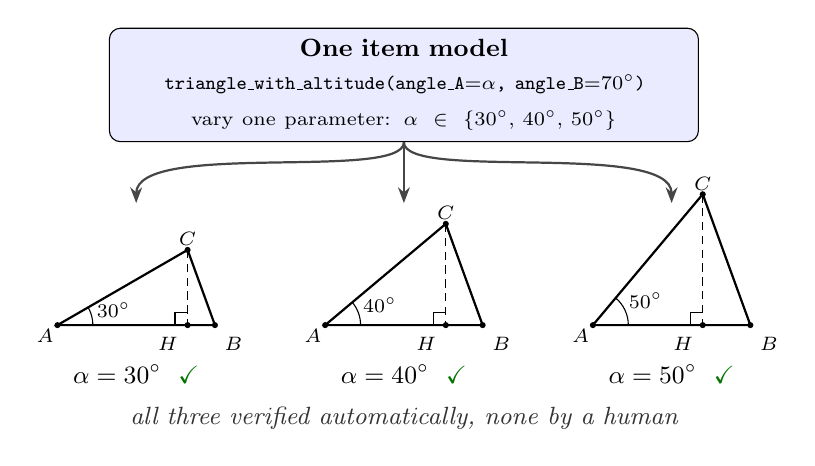
\begin{tikzpicture}[
    font=\small,
    tmpl/.style={draw, rounded corners, fill=blue!8, align=center,
                 text width=72mm, minimum height=11mm, inner sep=4pt},
    ar/.style={-{Stealth[length=2mm]}, thick, gray!55!black},
]
% --- the item model ---
\node[tmpl] (t) at (4.4,3.05) {\textbf{One item model}\\[1pt]
  {\scriptsize\ttfamily triangle\_with\_altitude(angle\_A${=}\alpha$,\ angle\_B${=}70^\circ$)}\\[2pt]
  {\scriptsize vary one parameter: $\alpha \in \{30^\circ,\,40^\circ,\,50^\circ\}$}};
% --- three generated instances ---
\foreach \sx/\cx/\cy/\ang in {0/1.653/0.955/30, 3.4/1.532/1.286/40, 6.8/1.395/1.662/50}{
  \begin{scope}[shift={(\sx,0)}]
    \coordinate (A) at (0,0); \coordinate (B) at (2,0);
    \coordinate (C) at (\cx,\cy); \coordinate (H) at (\cx,0);
    \draw[thick] (A)--(B)--(C)--cycle;
    \draw[densely dashed] (C)--(H);
    \draw (\cx-0.16,0)--(\cx-0.16,0.16)--(\cx,0.16); % right-angle mark at H
    \draw (0.45,0) arc (0:\ang:0.45);                % angle arc at A
    \node[font=\scriptsize] at (\ang/2:0.74) {$\ang^\circ$};
    \foreach \q in {A,B,C,H}{\fill (\q) circle (1.1pt);}
    \node[below left=-3pt, font=\scriptsize]  at (A) {$A$};
    \node[font=\scriptsize, anchor=north west] at ([yshift=-1pt]B) {$B$};
    \node[above=-2pt, font=\scriptsize]       at (C) {$C$};
    \node[font=\scriptsize, anchor=north east] at ([yshift=-1pt]H) {$H$};
    \node[font=\small] at (1,-0.62)
      {$\alpha=\ang^\circ$\ \ {\color{green!45!black}\checkmark}};
  \end{scope}
}
% --- fan-out arrows + verdict line ---
\foreach \sx in {0,3.4,6.8}{
  \draw[ar] (t.south) .. controls +(0,-0.5) and +(0,0.8) .. (\sx+1,1.55);}
\node[font=\small\itshape, color=gray!40!black] at (4.4,-1.18)
  {all three verified automatically, none by a human};
\end{tikzpicture}
\caption{From one item model to a family of verified items. This is automatic item generation with the answer key built in. Hold every parameter fixed but the angle at $A$ and sweep it through $30^\circ, 40^\circ, 50^\circ$. That produces parallel variants. For each, the checker of \cref{sec:scoring} confirms that the altitude from $C$ meets $AB$ at a right angle (\checkmark), with no human review. One model yields a refreshable supply of items, each carrying its own key.}
\label{fig:variants}
\end{figure*}

Each template is an item generator. Fixing every parameter but one and sweeping that parameter, for example an angle through $30^\circ, 40^\circ, 50^\circ$, produces a family of structurally parallel questions, and the checker confirms each variant without human review (\cref{fig:variants}). The answer key is produced \emph{with} each item rather than written afterward. So a common source of scoring error, a hand-written key that has drifted from its question, is largely designed out. In the vocabulary of the field the template is an \emph{item model} \citep{gierl2012itemmodels}, now one that emits its own key. That move also shifts where quality control happens, in the way the item-generation literature recommends. Rather than vetting every generated item, one reviews the construction logic that produces them all \citep{gierl2016review}.

The diagram a student (or a model) produces is a constructed response. The same description that built the item can score it. Here a measurement audience should consider two claims separately. The \emph{generation} claim rests on firmer ground. The key is computed with the item rather than written separately, so question and key are far less likely to drift apart. And the key is a short, readable list of exactly what must be true (\cref{tab:predicates}), open to inspection rather than embedded in a holistic rubric. The \emph{scoring} claim must be established empirically, and our validity study (\cref{sec:scoring}) shows that it is not yet established. The auto-score agrees with human graders only moderately and errs in a single direction. For now it is an optimistic estimate. That is fit for benchmarking and for flagging likely-wrong work. It is not yet fit for standalone high-stakes scoring. Closing that gap means adding the numeric checks that \cref{sec:scoring} pinpoints.

\paragraph{Three measurement questions the checklist opens.}
First, isomorphism. Variants minted from one item model are parallel in construction. Parallel construction does not guarantee equal difficulty. A $30^\circ$ angle may be harder to draw than a $50^\circ$ one. Whether the variants are true isomorphs is a calibration question. The framework makes that study inexpensive, because every variant comes with its key. Second, partial credit. The checker decides every requirement separately, so a score need not be all-or-nothing. A diagram that places the altitude correctly but misses the stated angle can earn credit for what it got right. The per-requirement verdicts provide the basis for a partial-credit rubric. The weights and score categories remain to be decided. Our graders also rated diagrams requirement by requirement. They agreed with the checker on 98\% of 864 individual ratings. The overall disagreement in \cref{sec:scoring} comes largely from requirements the checklist left out, not from the ones it contains. Third, the checklist as a Q-matrix. Each item's list of checks names the geometric requirements the item imposes, in a fixed vocabulary shared across items. That is the raw form of a Q-matrix, the item-by-attribute table a cognitive diagnostic model needs. Mapping requirements to the skills a student uses still takes judgment and empirical validation. But an initial version of the table is produced by the item model rather than coded by hand afterward.

\paragraph{Scope.}
The version described here covers plane geometry. The same machinery should extend to coordinate graphs and 3D solids by adding new kinds of building block. We have not built those yet. Where a topic has no natural template, an author can still write items and keys by hand and score them with the same checker. The core idea is simple. When a diagram is built from a structured description, that description says what must be checked, and a machine can check it. Whether the description is complete is a question for validation, and \cref{sec:scoring} shows why.


\bibliography{refs}

\end{document}
